
\section{Configuración experimental}


La metodología propuesta sigue  un enfoque supervisado, tal como se ilustra en la figura \ref{fig:metodologia}. En la cual se cuenta con un conjunto de datos $X$ con su etiqueta correspondiente $y \in Y$  en una relación uno a uno. El aumento de datos propuesto se realiza como una segunda etapa de preprocesamiento solo sobre los datos destinados al entrenamiento.

Dentro de la metodología empleada existen 4 fases:  preprocesamiento, aumento de datos, entrenamiento y evaluación. En el pre-procesamiento se realizan las modificaciones necesarias para normalizar el texto, posteriormente se puede construir un modelo de aprendizaje sin aumento de datos, sin embargo no se puede construir un modelo de aprendizaje sin los datos originales etiquetados. El paso final es la evaluación, la cual se realiza sobre un conjunto de datos que no es aumentado ni utilizado en la búsqueda de parámetros o durante el entrenamiento, solo es preprocesado de la misma forma que los datos originales.

%[!htbp]
\begin{figure}[h]
    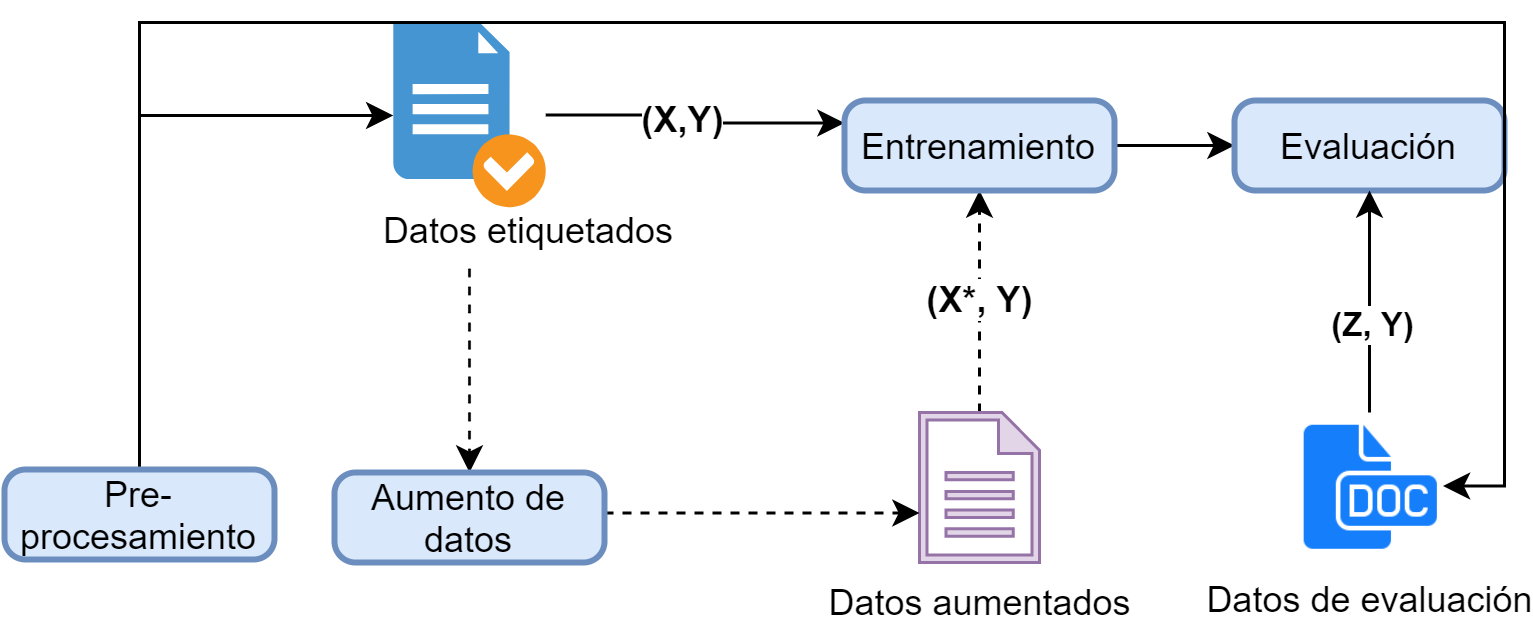
\includegraphics[width=\textwidth]{sections/figures/methodposter.png}
    \caption{Metodología de aumento de datos supervisada}
    \label{fig:metodologia}
\end{figure}

\subsection{Conjunto de datos}


Con el propósito de estudiar la detección temprana de depresión y anorexia, los autores \cite{Losada2018} recopilaron publicaciones de diversos usuarios de la red social Reddit. Para cada usuario la colección contiene una secuencia de publicaciones en orden cronológico. Este conjunto de datos se caracteriza por tener una gran cantidad de texto pero con muy pocos usuarios, como se puede observar en la figura \ref{fig:erisk_freq}. Hay dos categorías para cada usuario en cada tarea. El número de usuarios total en cada conjunto se presenta en la tabla \ref{table:users}. Dado que se trabaja con conjuntos de datos muy desbalanceados el aumento de datos solo se aplica sobre la clase de interés o clase positiva.

\begin{table}[!hbt]
\caption{Número de usuarios en los conjuntos de datos y número de sub-documentos con 64 palabras después del pre-procesamiento, sin aplicar el filtro de sub-documentos.} \label{table:orginal_users}
\begin{center}

\begin{tabular}{llll}
\hline
\rowcolor[HTML]{FFFFFF} 
\textbf{Usuarios}                                           & \textbf{Entrenamiento}                       & \textbf{Evaluación}                          & \textbf{Vocabulario}                                         \\ \hline
\rowcolor[HTML]{EFEFEF} 
\textit{Conjunto 1: Depresión 2018}                         & \multicolumn{1}{c}{\cellcolor[HTML]{EFEFEF}} & \multicolumn{1}{c}{\cellcolor[HTML]{EFEFEF}} &                                                              \\ \hline
\rowcolor[HTML]{FFFFFF} 
deprimido                                                   & 135 - 31,396                                 & 79 - 25,967                                  &                                                              \\ \hline
\rowcolor[HTML]{FFFFFF} 
no-deprimido                                                & 752 - 227,189                                & 741 - 272,703                                &                                                              \\ \hline
\rowcolor[HTML]{FFFFFF} 
\textbf{Total}                                              & \textit{887 - 138,232}                       & \textit{820 - 298,670}                       & \multicolumn{1}{c}{\cellcolor[HTML]{FFFFFF}\textit{202,151}} \\ \hline
\rowcolor[HTML]{EFEFEF} 
\cellcolor[HTML]{EFEFEF}\textit{Conjunto 2: Depresión 2019} &                                              &                                              &                                                              \\ \hline
\rowcolor[HTML]{FFFFFF} 
deprimido                                                   & 16 - 5,731                                   & 60 - 18,534                                  &                                                              \\ \hline
\rowcolor[HTML]{FFFFFF} 
no-deprimido                                                & 752 - 227,189                                & 10 - 5,011                                   &                                                              \\ \hline
\rowcolor[HTML]{FFFFFF} 
\textbf{Total}                                              & \textit{768 - 232,920}                       & \textit{70 - 23,545}                         & \multicolumn{1}{c}{\cellcolor[HTML]{FFFFFF}\textit{195,047}}    \\ \hline
\rowcolor[HTML]{EFEFEF} 
\textit{Conjunto 3: Anorexia}                               & \multicolumn{1}{c}{\cellcolor[HTML]{EFEFEF}} & \multicolumn{1}{c}{\cellcolor[HTML]{EFEFEF}} &                                                              \\ \hline
\rowcolor[HTML]{FFFFFF} 
con anorexia                                                & 61 - 23,335                                  & 73 - 16,751                                  &                                                              \\ \hline
\rowcolor[HTML]{FFFFFF} 
sin-anorexia                                                & 411 - 36,484                                 & 742 - 254,640                                &                                                              \\ \hline
\rowcolor[HTML]{FFFFFF} 
\textbf{Total}                                              & \textit{472 - 130,574}                       & \textit{815 - 271,391}                       & \multicolumn{1}{c}{\cellcolor[HTML]{FFFFFF}\textit{67,724}}  \\ \hline
\end{tabular}

\end{center}

\end{table}




%[!htbp]
\begin{figure}[!ht]
    
    \begin{subfigure}[b]{0.5\textwidth}
        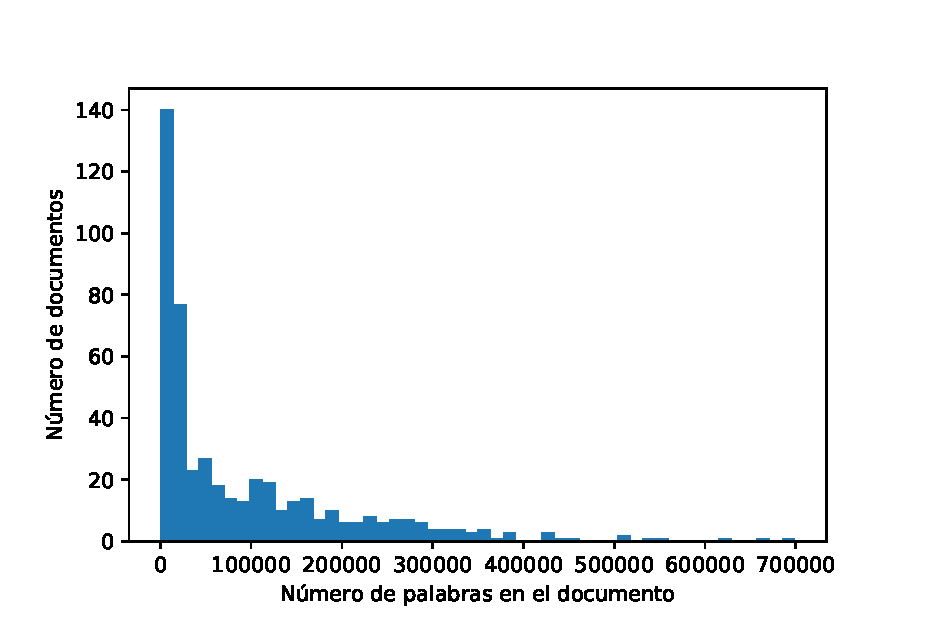
\includegraphics[width=\textwidth]{sections/figures/length_dist.eps}
        \caption{Depresión}
    \end{subfigure}
    \hfill
    \begin{subfigure}[b]{0.5\textwidth}
        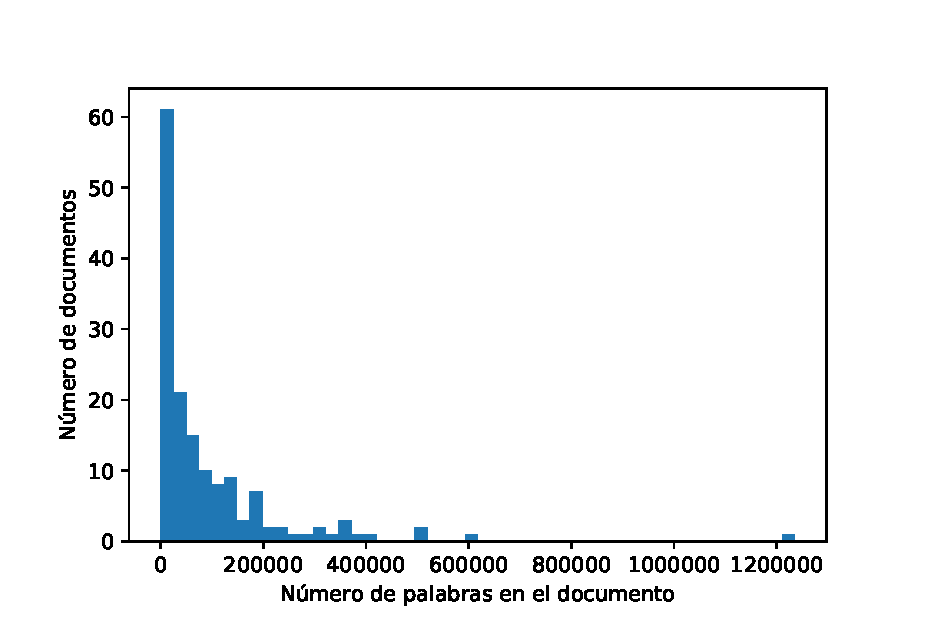
\includegraphics[width=\textwidth]{sections/figures/length_dist_anorexia.eps}
        \caption{Anorexia}
    \end{subfigure}
    \caption{Distribución del numero de palabras en los conjuntos de datos estudiados}
    \label{fig:erisk_freq}
\end{figure}

%% Agregar las distribución del conjunto anorexia


\subsection{Pre-procesamiento}

Dado que los documentos extraídos de redes sociales no siguen un lenguaje formal y además de texto existen direcciones de páginas web que los usuarios comparten, emoticonos y cáracteres especiales, entre otros; es necesario que antes del aumento de datos exista un preprocesamiento de los textos como una forma de reducir el ruido de los documentos originales.

Los pasos del procesamiento seguido son los siguientes:

 \begin{enumerate}
     \item Normalización: Se identifican las páginas web en el texto y se reemplazan mediante la etiqueta http\_
     \item Tokenización: Utilizando la herramienta NLTK se remueve de cada texto signos de puntuación y cáracteres especiales.
     \item Segmentación: Para que el aumento de datos sea similar para cada documento, cada historial de usuario se divide en secuencias de 64 palabras. 
     %\item Filtro: En la clasificación de documentos no todo el contenido del texto esencial para determinar la categoría a la cual pertenece, es decir existe cierta combinación de palabras que sirven para discriminar la clase. Para determinar estas palabras se emplea el método de selección de características denominado Chi-cuadrada.
     \item Filtro: Solo se conservan segmentos indentificados como importantes para la clasificación.
 \end{enumerate}



\subsubsection{Segmentación y filtro}
Con el objetivo de que el aumento de datos pueda ser proporcional independientemente de la longitud del documento original. Cada documento se dividió en segmentos de 64 palabras. Posteriormente se filtró el conjunto de entrenamiento para conservar solo los segmentos más importantes para la clasificación, esto se realiza seleccionando las palabras más discriminantes dentro del vocabulario del conjunto de entrenamiento mediante la técnica de selección de características $\chi^2$, posteriormente se filtran los segmentos que contengan un determinado número de palabras con alta puntuación $\chi^2$. 

Específicamente solo se seleccionaron términos estadísticamente significativos al nivel 0.001, equivalente a una puntuación $\chi^2 > $ 10.83 con un grado de libertad. En la tabla \ref{table:filter_users} se muestran los números de usuarios y secuencias obtenidas después de aplicar este filtro; para el conjunto de depresión el criterio de selección fue que la secuencia contuviera al menos 20 palabras de 1071 palabras con alta puntuación, y para el conjunto de anorexia 15 palabras de 1032. La razón de utilizar números altos es debido a que también se están considerando palabras de paro.

\begin{table}[!hbt]
\caption{Número de usuarios en los conjuntos de datos y número de secuencias con 64 palabras después del pre-procesamiento, realizando el filtro. Los números resaltados en negritas representan el numero de historiales comparado con el numero de secuencias} \label{table:filter_users}

\resizebox{\textwidth}{!}{%

\begin{tabular}{llll}
\hline
\rowcolor[HTML]{FFFFFF} 
\textbf{Usuarios}                   & \textbf{Entrenamiento}                       & \textbf{Evaluación}                          & \textbf{Vocabulario}                                         \\ \hline
\rowcolor[HTML]{EFEFEF} 
\textit{Conjunto 1: Depresión 2018} & \multicolumn{1}{c}{\cellcolor[HTML]{EFEFEF}} & \multicolumn{1}{c}{\cellcolor[HTML]{EFEFEF}} &                                                              \\ \hline
\rowcolor[HTML]{FFFFFF} 
deprimido                           & \textbf{135} - 24,483                                 & \textbf{79} - 25,967                                  &                                                              \\ \hline
\rowcolor[HTML]{FFFFFF} 
no-deprimido                        & \textbf{744} - 98,783                                 & \textbf{741} - 272,703                                &                                                              \\ \hline
\rowcolor[HTML]{FFFFFF} 
\textbf{Total}                      & \textit{\textbf{879} - 123,266}                       & \textit{\textbf{820} - 298,670}                       & \multicolumn{1}{c}{\cellcolor[HTML]{FFFFFF}\textit{104,800}} \\ \hline
\rowcolor[HTML]{EFEFEF} 
\textit{Conjunto 2: Depresión 2019} & \multicolumn{1}{c}{\cellcolor[HTML]{EFEFEF}} & \multicolumn{1}{c}{\cellcolor[HTML]{EFEFEF}} &                                                              \\ \hline
\rowcolor[HTML]{FFFFFF} 
deprimido                           & \textbf{16} - 5,731                                   & \textbf{60} - 18,534                                  &                                                              \\ \hline
\rowcolor[HTML]{FFFFFF} 
no-deprimido                        & \textbf{746} - 125,823                                & \textbf{10} - 5,011                                   &                                                              \\ \hline
\rowcolor[HTML]{FFFFFF} 
\textbf{Total}                      & \textit{\textbf{762} - 131,554}                       & \textit{\textbf{70} - 23,545}                         & \multicolumn{1}{c}{\cellcolor[HTML]{FFFFFF}\textit{118,668}}    \\ \hline
\rowcolor[HTML]{EFEFEF} 
\textit{Conjunto 2: Anorexia}       & \multicolumn{1}{c}{\cellcolor[HTML]{EFEFEF}} & \multicolumn{1}{c}{\cellcolor[HTML]{EFEFEF}} &                                                              \\ \hline
\rowcolor[HTML]{FFFFFF} 
con anorexia                        & \textbf{61}-23,335                                    & \textbf{73}-16,751                                    &                                                              \\ \hline
\rowcolor[HTML]{FFFFFF} 
sin-anorexia                        & \textbf{411}-107,239                                  & \textbf{742}-254,640                                  &                                                              \\ \hline
\rowcolor[HTML]{FFFFFF} 
\textbf{Total}                      & \textit{\textbf{472}-130,574}                         & \textit{\textbf{815}-271,391}                         & \multicolumn{1}{c}{\cellcolor[HTML]{FFFFFF}\textit{131,264}} \\ \hline
\end{tabular}

}

\end{table}


\subsection{Configuración del método propuesto}

Para comprobar la efectividad del método propuesto se experimenta con  7 configuraciones diferentes: 2 líneas base, 2 métodos del estado del arte y 3 métodos propuestos. Además de esto se introduce un parámetro $n$ para observar el grado pertinente del aumento de datos, el cual indica el número de documentos nuevos, tomando valores enteros en el rango $[1,10]$.

% \begin{enumerate}
%     \item Sin aumento de datos:
%     \item Sobre muestreo:
%     \item Sustitución sin restricción.
%     \item Restricción Chi cuadrado.
%     \item Reemplazo mediante relaciones de la misma clase:
%     \item Reemplazo mediante relaciones de la clase contraria.
% \end{enumerate}


\subsubsection{Sin aumento de datos}
Este método es la primera línea base y solo consideran los datos originales filtrados para el entrenamiento de los modelos (véase la tabla \ref{table:filter_users}).

\subsubsection{Sobre muestreo}
Esta línea base, consiste en incrementar el número de ejemplos de la clase minoritaria; este método no implica alguna perdida de información ya que ningún elemento es modificado o descartado. Sin embargo la única desventaja es, que el modelo de aprendizaje generado tiende a sobre ajustarse, debido a que no agrega variabilidad en los datos.

\subsubsection{Tesauro}
Este método del estado del arte fue propuesto por \cite{zhang2015character} y demostró mejoras de un 1 a 2\% en exactitud para la clasificación de opiniones. También fue implementado por \cite{wei2019eda} con algunas modificaciones obteniendo una mejora entre un 1 y 2\% en comparación de no hacer aumento de datos, otros trabajos que utilizan este método como referencia y han encontrado evidencia de que agrega una ganancia en los resultados de clasificación son: \cite{jungiewicz2019towards}, \cite{kumar2019submodular}, \cite{park2019self}.

De acuerdo a la figura \ref{fig:aumento}, en la fase de selección se utiliza el parámetro $p=$ 0.5 para calcular el valor de $r$ palabras a reemplazar, la selección de dichas palabras es aleatoria, el recurso externo para encontrar sinónimos es un tesauro (en este caso Wordnet\footnote{www.wordnet.princeton.edu/}), y finalmente en la fase de reemplazo, de las palabras candidatas, se selecciona el índice dado un número aleatorio $s$ generado de una distribución geométrica con parámetro $q=$ 0.5.

El propósito de este método es ser muy conservativo en la modificación del texto original y el número $s$ controla la diversidad del vocabulario que por lo general siempre será la primer palabra de las candidatas (la más empleada).

\subsubsection{Sustitución sin restricción y reemplazo mediante similitud coseno}
Diversos estudios sugieren utilizar vectores de modelos pre-entrenados como Word2Vec, Glove, entre otros; la idea es recuperar palabras que se utilizan en contextos similares, en lugar de sinónimos. 

Este método sigue el esquema de la figura \ref{fig:aumento}, en la fase de selección solo se omiten palabras de paro y aquellas que no sean etiquetadas como sustantivos, adjetivos, verbos y adverbios; el número $r$ es calculado con el parámetro $p=$ 0.2. En la fase de reemplazo las palabras más similares se seleccionan mediante similitud coseno, utilizándolas de mayor a menor en una selección sin reemplazo.

El modelo de vectores pre-entrenados fue Glove\footnote{https://nlp.stanford.edu/projects/glove/} con 300 dimensiones \cite{pennington2014glove}. Este modelo fue pre-entrenado con la base de datos Common Crawl, con 42 millones de  tokens y 1.9 millones de palabras. 

%no separar vocales
Con este método se espera obtener mayor diversidad en el vocabulario en comparación a utilizar un tesauro y obtener palabras muy similares que se emplean en el mismo contexto.

\subsubsection{Sustitución con restricción $\chi2$  y reemplazo mediante similitud relacional}
A diferencia del método anterior, una vez calculado el número $r$ de palabras a reemplazar, se omiten las palabras con mayor puntuación $\chi^2$ con un nivel de significación estadística de 0.001. Con este método se espera conservar una combinación de estilo y contenido además de agregar variabilidad en los datos.

\subsubsection{Reemplazo mediante similitud relacional equivalente}
En la fase de selección se fija el valor del parámetro $p=$ 0.2 y en la fase de reemplazo se utiliza la similitud relacional positiva; esto es obtener un vocabulario muy similar a la etiqueta de la clase pero no el mismo. Las relaciones buscadas se listan en la tabla \ref{table:etiquetas} para cada conjunto de datos. Por ejemplo para buscar las palabras candidatas a la palabra ``boyfriend", se utiliza la relación \textit{``depressed"} es a \textit{``boyfriend"} como \textit{``anxious"} es a \textbf{?}. 

\subsubsection{Reemplazo mediante similitud relacional contraria}
Muy similar al método anterior lo único que cambia es la clase objetivo, en este caso se toman los documentos de clase contraria (la clase negativa) y se aumentan de acuerdo al método propuesto en la figura \ref{fig:aumento}. Por ejemplo para buscar las palabras candidatas a la palabra ``boyfriend", se utiliza la relación \textit{``happiness"} es a \textit{``boyfriend"} como \textit{``anxious"} es a \textbf{?}. La tabla \ref{table:etiquetas} resume las etiquetas empleadas para realizar el aumento.


\begin{table}[!hbt]
\caption{Etiquetas utilizadas en el proceso de aumento para los métodos de similitud relacional.} \label{table:etiquetas}
\begin{center}

\begin{tabular}{llll}
\hline
\rowcolor[HTML]{C0C0C0} 
Conjunto           & Clase & Etiqueta  & Palabra relacionada \\ \hline
\textbf{Depresión} & 1     & depressed & anxious           \\ \hline
                   & 0     & happiness & frustrated        \\ \hline
                   &       &           & unhappy           \\ \hline
                   &       &           & despondent        \\ \hline
                   &       &           & discouraged       \\ \hline
\textbf{Anorexia}  & 1     & anorexic  & bulimic           \\ \hline
                   & 0     & healthy   & underweight       \\ \hline
                   &       &           & obese             \\ \hline
                   &       &           & malnourished      \\ \hline
                   &       &           & unhealthy         \\ \hline
\end{tabular}

\end{center}
\end{table}


 
\subsection{Configuración del modelo de aprendizaje}

Para demostrar el efecto del aumento de datos tanto en modelos de aprendizaje basados de redes neuronales como en modelos tradicionales lineales (SVM). Se implementa una máquina de soporte vectorial SVM y una SVM-C. Además de una red LSTM bidireccional y una red convolucional CNN con el principal objetivo de contrastar el impacto del aumento de datos, cuando se considera el texto secuencial en el caso de la red recurrente y cuando se consideran las características como elementos aislados en el caso de la red convolucional.

\subsubsection{Modelos lineales}
 El primer modelo es construido mediante una Máquina de Soporte Vectorial (SVM) con kernel lineal, la entrada es el historial completo de un usuario representado como un vector de características mediante el pesado \textit{tf-idf} y normalizado mediante la norma $l2$, las palabras de paro se mantienen y se utiliza todo el vocabulario extraído como características. 
 
 El segundo algoritmo utilizado, SVM-C,  es basado en el primer modelo, con la diferencia de que en este caso se modifica el parámetro de regularización $C$ y automáticamente se ajustan los pesos inversamente proporcional a la frecuencia de las clases en los datos de entrada de acuerdo la ecuación \ref{eq:weights_balance}
 
 \begin{equation}
 \label{eq:weights_balance}
     C = N/2c_n
 \end{equation}
 
 En donde $N$ es el número total de ejemplos y $c_n$ el número de ejemplos en la clase $c$.  

\subsubsection{Modelos basados en redes neuronales}

Con el objetivo principal de establecer las bases sobre en que tipo de arquitecturas es más recomendable realizar aumento de datos. Se implementan dos arquitecturas diferentes: una red Bidireccional LSTM (Bi-LSTM) y una red convolucional (CNN); teniendo en común la capa de entrada y capa de salida.

La \textbf{capa de entrada} recibe una secuencia de 64 palabras, cada palabra es representada por un vector de 300 dimensiones obtenido del modelo pre-entrenado FastText\footnote{https://fasttext.cc/docs/en/crawl-vectors.html} , si alguna palabra no está en el vocabulario, su vector es obtenido de la representación de sus n-gramas de caracteres. En el entrenamiento esta capa es estática para reducir el número de parámetros entrenables.

La \textbf{capa de salida} es una neurona que recibe como entrada la última capa oculta del modelo, la representación aprendida de los parámetros internos. Mediante la función sigmoide, ecuación \ref{eq:sigmoide}, se calcula la probabilidad de que la secuencia de palabras pertenezca a la clase 0 o a la clase 1.

\begin{equation}
    \label{eq:sigmoide}
    sigmoid(x) = \frac{1}{1+ e^{-x}}
\end{equation}

Para inicializar los pesos de la capa final correctamente, el \textit{bias} (sesgo) inicial se deriva de la ecuación \ref{eq:bias}.  Con la inicialización correcta la función de perdida inicial se debe aproximar a $ln(2)=$ 0.69314. 

\begin{equation}
\label{eq:bias}
\begin{split}
    p_0= \frac{pos}{pos+neg}= \frac{1}{1+e^{-b_0}}\\
    b_0=-log_e(\frac{1}{p_0-1})\\
    b_0=log_e(pos/neg)
\end{split}
\end{equation}

Configurando el sesgo inicial correctamente ayuda a la convergencia del modelo desde la primer época.

%%No se puede dividir poster
%Agregar referencia y cambiar figura 
Derivado de la arquitectura presentada en  \cite{adhikari2019rethinking}, en la figura  \ref{fig:lstm_model}, se presenta la arquitectura empleada para el modelo Bi-LSTM, la red bidireccional se compone de dos redes LSTM con 256 neuronas cada una, posteriormente de aplica una capa de \textit{Dropout} con una tasa de 0.2 , una capa totalmente conectada con 256 unidades, una capa de \textit{Dropout} con una tasa de 0.2 y en la última capa una sola neurona activada mediante la función sigmoide \ref{eq:sigmoide}. Los nodos intermedios de las capas ocultas se activan con la función de activación Relu \ref{eq:RELU}. 
\begin{figure}[!hb]
    \centering
  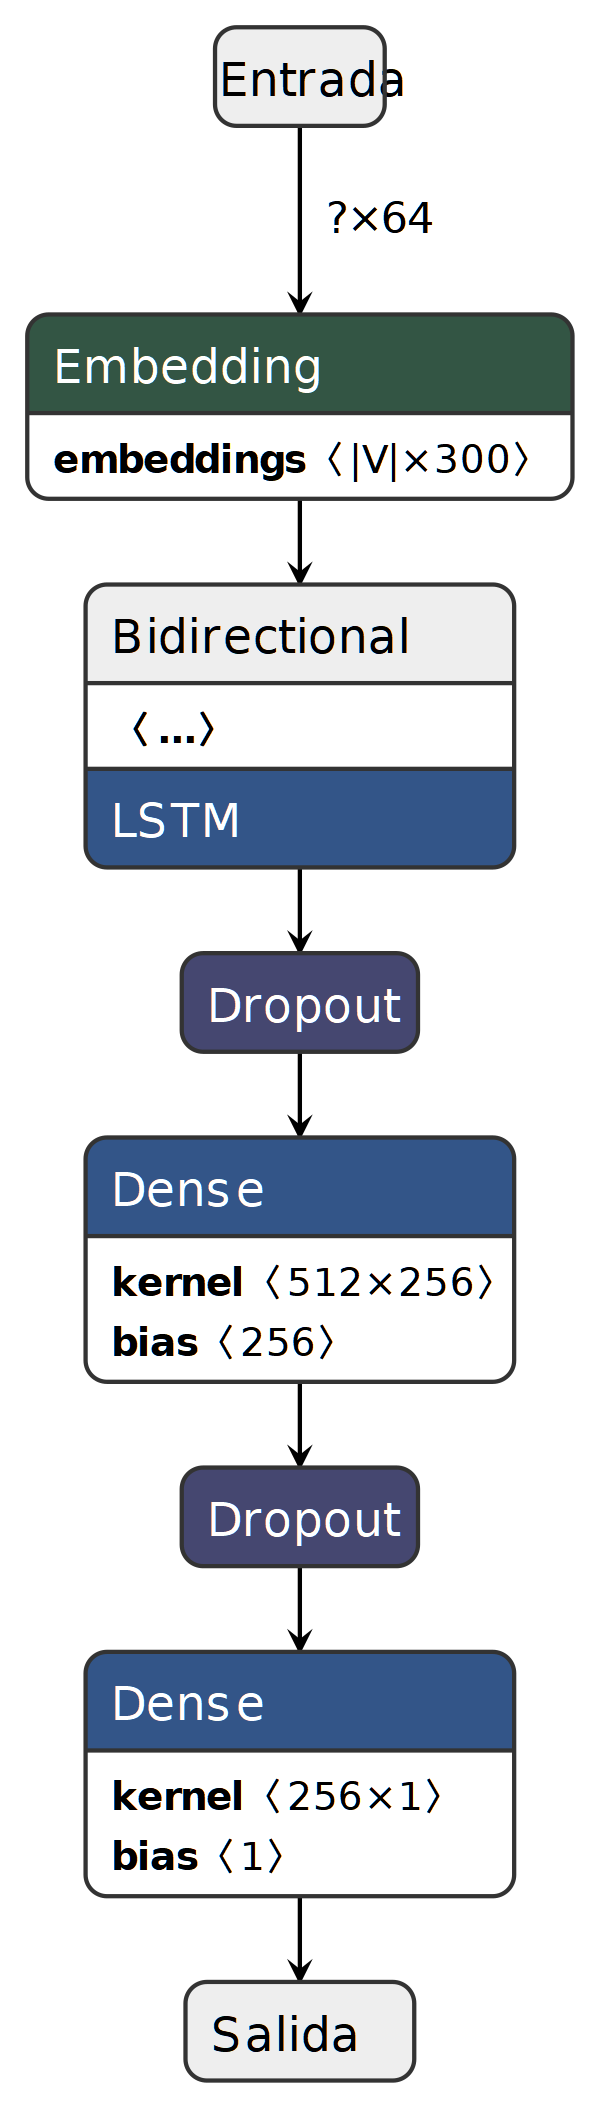
\includegraphics[scale=0.25]{sections/figures/lstm_model.png}
    \caption{Arquitectura del modelo Bi-LSTM}
    \label{fig:lstm_model}
\end{figure}

%%Elminar 

En la figura \ref{fig:cnn_model}, se presenta la arquitectura empleada para la red convolucional (CNN), esta arquitectura es basada en el trabajo de \cite{kim2014convolutional}. Se implementan tres tamaños de filtro [3,4,5], cada uno con 300 filtros. Los filtros realizan convoluciones en una matriz que representa a la secuencia de palabras y generan mapas de características de longitud variable; la operación de \textit{Max Pooling }se realiza sobre cada mapa, es decir, se calcula el número mayor de cada mapa de características. A partir de esto se obtienen diferentes vectores de características de diferentes tamaños y la penúltima capa se forma concatenándolos para formar un vector final de características, la capa final recibe este vector de características para clasificar la secuencia de palabras. Los nodos intermedios de las capas ocultas se activan con la función de activación Relu \ref{eq:RELU}. 

\begin{figure}[!h]
    \centering
  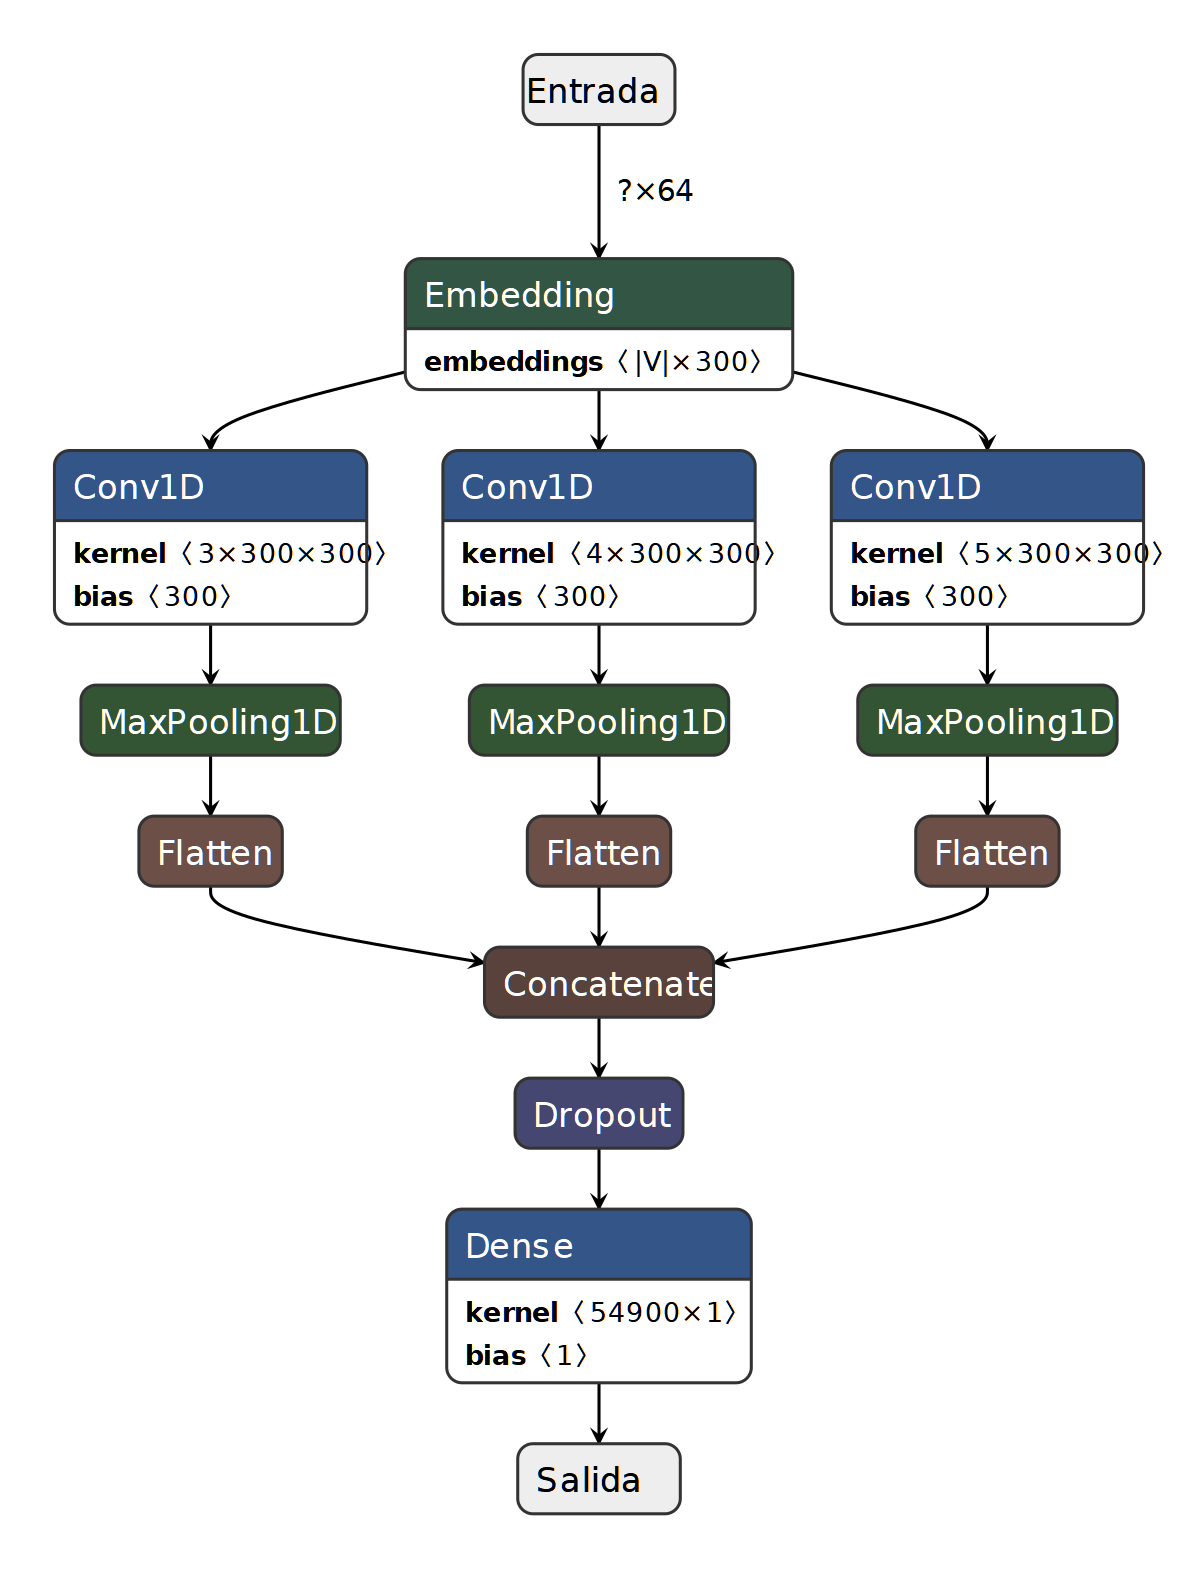
\includegraphics[scale=0.3]{sections/figures/cnn_model.png}
    \caption{Arquitectura del modelo CNN con múltiples tamaños de convolución}
    \label{fig:cnn_model}
\end{figure}


\subsubsection{Entrenamiento}
Para encontrar los hiperparámetros de los modelos se realizó una división del conjunto de entrenamiento en 3 particiones diferentes (3 K-Folds) con una proporción de 66\% para entrenar y 33\% para evaluar.

En el caso de los modelos de redes neuronales se entrenan de forma que sean sensibles al desbalance \cite{wang2016training}, utilizando un peso adicional para cada clase, calculado mediante la fórmula \ref{eq:weights_balance}. Con esto el error es incrementado para ejemplos en la clase de interés y decrementado para la clase menos importante.

Los parámetros elegidos para el entrenamiento se resumen en la tabla \ref{table:param_redes}. Al finalizar el entrenamiento la predicción final se realiza reuniendo todos los segmentos del usuario a identificar y mediante un intérvalo de confianza se puede decidir si pertenece a la clase positiva o negativa.


\begin{table}[t]
\caption{Parámetros utilizados para el entrenamiento de los modelos basados en redes neuronales.} \label{table:param_redes}
\begin{center}

\begin{tabular}{lc}
\hline
\rowcolor[HTML]{C0C0C0} 
\textbf{Parámetro}      & \textbf{Valor}           \\ \hline
Tasa de aprendizaje     & 1.00E-03                 \\ \hline
Tamaño del Batch        & 1024                     \\ \hline
Función de pérdida      & Entropia cruzada binaria \\ \hline
Máximo número de epocas & 20                       \\ \hline
Criterio de paro    & CNN=6; Bi-LSTM=3         \\ \hline
Pruebas independientes  & 3                        \\ \hline
\end{tabular}

\end{center}
\end{table}

\subsubsection{Implementación}
Para el preprocesamiento y el etiquetado de las secuencias de texto se utilizó la librería NLTK \cite{loper2002nltk}, para la normalización y el cálculo de medidas de similitud de los embeddings la librería gemsin\footnote{www.radimrehurek.com/gensim}.
Los modelos lineales fueron implementados utilizando la librería sckit-learn\footnote{www.scikit-learn.org/stable/} \cite{scikitlearn}, los modelos neuronales\footnote{www.tensorflow.org} \cite{tensorflow2015whitepaper}. Todas en su última versión mediante en el lenguaje de programación Python.
